\documentclass[12pt,a4paper]{article}
\usepackage[utf8]{inputenc}
\usepackage[L7x]{fontenc}
\usepackage[lithuanian]{babel}
\usepackage{lmodern} %be neveikia bold, italic etc

\usepackage{amsmath}
\usepackage{amsfonts}
\usepackage{amssymb}

\usepackage{float} %galima naudoti [H] kad būtų ten, kur reikia pav, table etc

\usepackage{hyperref} %naudojami linkai veikia


\usepackage{graphicx}
\graphicspath{{./figures/}}

\usepackage{listings}
\usepackage{color}
\usepackage{textcomp}
\definecolor{listinggray}{gray}{0.9}
\definecolor{lbcolor}{rgb}{0.9,0.9,0.9}
\lstset{
	backgroundcolor=\color{lbcolor},
	tabsize=4,
	rulecolor=,
	language=html,
	 commentstyle=\color{mygreen},
        basicstyle=\scriptsize,
        upquote=true,
        aboveskip={0.5\baselineskip},
        belowskip={0.5\baselineskip},
        columns=fixed,
        showstringspaces=false,
        extendedchars=false,
        breaklines=true,
        prebreak = \raisebox{0ex}[0ex][0ex]{\ensuremath{\hookleftarrow}},
        frame=single,
        showtabs=false,
        showspaces=false,
        showstringspaces=false,
        identifierstyle=\ttfamily,
        keywordstyle=\color[rgb]{0,0,1},
        commentstyle=\color[rgb]{0.133,0.545,0.133},
        stringstyle=\color[rgb]{0.627,0.126,0.941},
        numbers=left,
        numbersep=5pt
}
\lstset{literate=
  {Č}{{\v{C}}}1 {Š}{{\v{S}}}1
}


\author{Justas Mundeikis\thanks{justas.mundeikis@evaf.vu.lt}}
\title{1 Seminaras}


\begin{document}
\maketitle
\section{Programų instaliavimas}
Instaliuokite šias programas savo asmeniniame kompiuteryje. Jeigu naudojatės VU kompiuteriais, gali prireikti instaliuoti nešiojamą (portable) versiją Sublime.

\begin{enumerate}
\item Instaliuokite R
\item Instaliuokite RStudio
\item Instaliuokite GitBash
\item Instaliuokite Sublime
\item Nepamirškite pagrindinių nustatymų
\begin{lstlisting}
$ git config --global user.name "Vardas Pavadre"
$ git config --global user.email vardas.pavarde@evaf.vu.lt
\end{lstlisting}
\end{enumerate}

\section{Paskyrų susikūrimas}
\begin{enumerate}
\item Susikurkite savo paskyrą, naudodami bet kokį pseudonimą @Github, tačiau naudodami savo universitetinį email vardas.pavarde@stud.vu.lt
\end{enumerate}

\section{Nuosavo tinklapio sukūrimo projektas}
Šioje dalyje naudosimės Git, Sublime ir Github, jog sukurti savo nuosavą internetinį puslapį. 
\\Pastaba: Tarkime, kad mano studento nr yra "S175", Jūsų gali būti kitoks, tada naudojate savo vietoj mano "S175"

\begin{enumerate}
\item Su Git nueiname and Desktopo (arba tiesiog paleidžiama "Git Bash Here" [su dešiniu pelės mygtuku])
\item Sukuriame folderį webpage \colorbox{listinggray}{\lstinline|mkdir -p S175/webpage|}
\item Perėjus į patį webpage folderį, inicijuojame jį su git, taigi prima \colorbox{listinggray}{\lstinline|cd S175/webpage|}, o tada \colorbox{listinggray}{\lstinline|git init|}
\item Pirmas dalykas, kurį mums reiktų sukurti, tai bazinis html dokumentas kurio pavadinimas būtų \textit{index} \colorbox{listinggray}{\lstinline|touch index.html|}
\item Jeigu tiesiog atsidarysite index.html failą su kuria nors naršykle, pamatysite, kad viskas yra absoliučiai balta! Neįdomu :D
\item Atsidarome \textit{index.html} su \textit{Sublime} editoriumi
\item Editoriuje įrašome tekstą
\begin{lstlisting}
Čia kuriamas mano tinklapis
\end{lstlisting}
išaugome (ctrl+s)
\item Atnaujiname interneto naršyklę (F5), rezultatas turėtų atrodyti daugmaž taip

\begin{figure}[ht]
\center
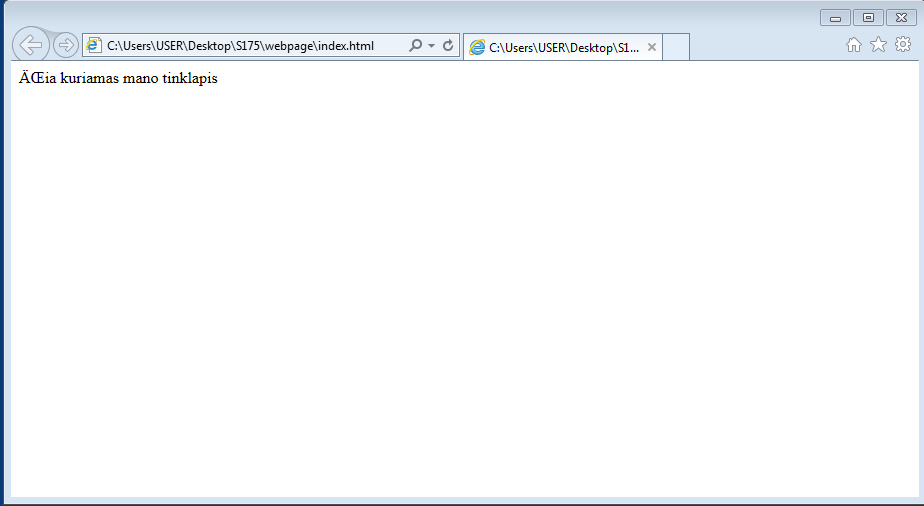
\includegraphics[scale=0.3]{webpage_1.png}
\end{figure}

\item Tam kad dokumentas turėtų antraštę, į pirmą eilutę parašom \colorbox{listinggray}{\lstinline|<h1> S175 tinklapis <\h1>|}. HTML kode \colorbox{listinggray}{\lstinline|<h1>|} pažymį pimro lygio antraštės \textit{tag}. Tiesa, \textit{Sublime} yra pakankamai protingas ir pradėjus rašyti <h išmeta pasirinkimą, pasirinkus h1 pats supildo viską, bereikia įrašyti tik savo tekstą
\begin{figure}[ht]
\center
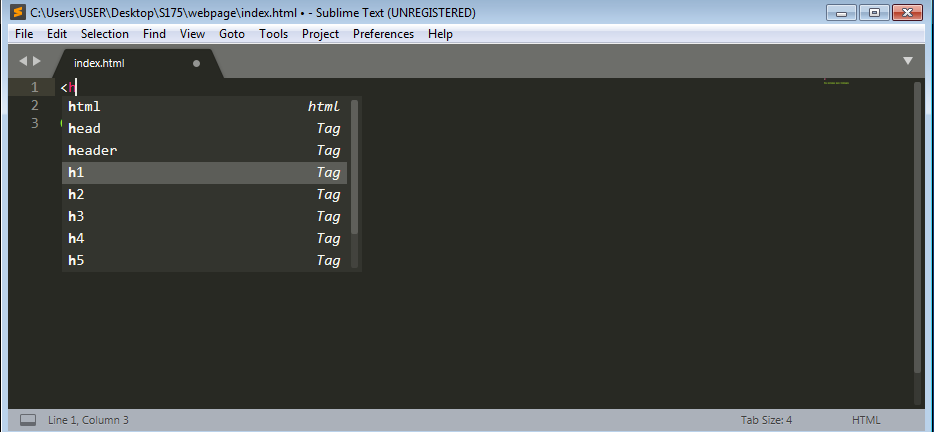
\includegraphics[scale=0.3]{webpage_2.png}
\end{figure}

\item Išsaugokite pakeitimus editoriuje ir atnaujinkite naršyklę

\begin{figure}[ht]
\center
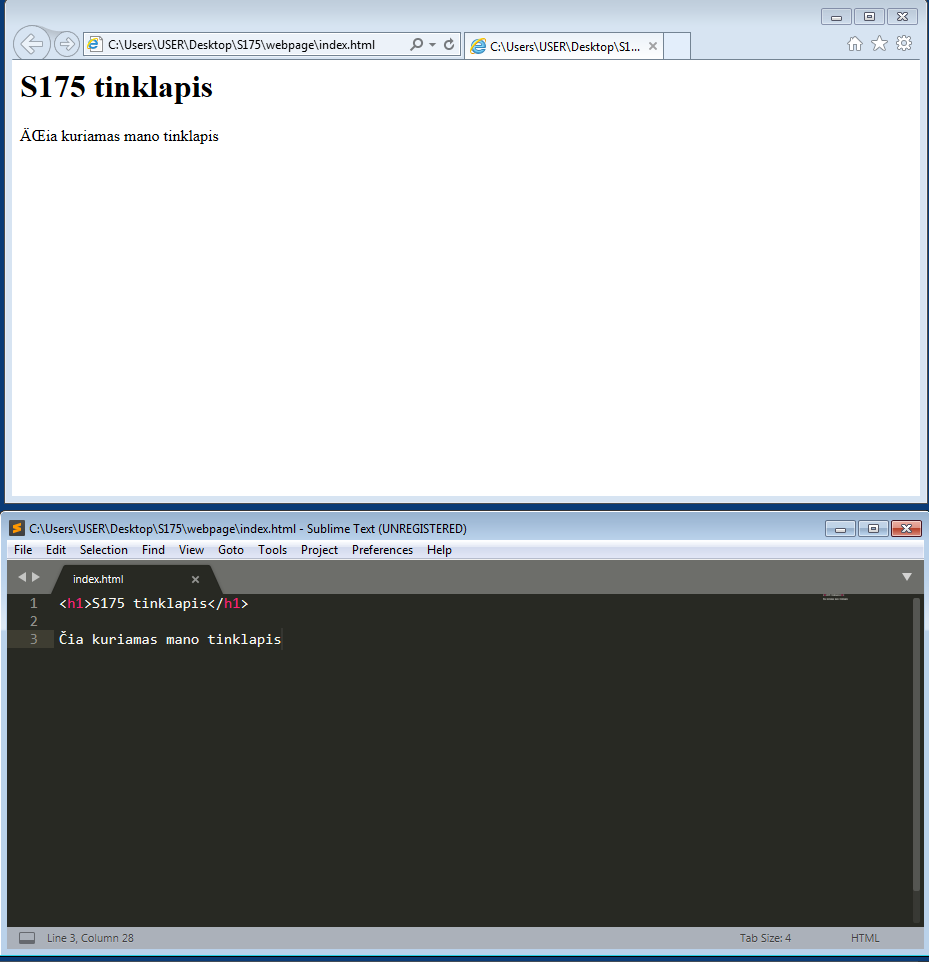
\includegraphics[scale=0.3]{webpage_3.png}
\end{figure}

\item \colorbox{listinggray}{\lstinline|git add . && git commit -m "Sukuriamas index.html failas"|}

\item Dabar prikurkime šiek tiek teksto mūsų tinklapiui pvz., "Šio tinklapio kūrimas yra  1.Seminaro darbas" ir išsaugome editoriaus pakeitimus

\begin{lstlisting}
<h1>S175 tinklapis</h1>

Čia kuriamas mano tinklapis

Šio tinklapio kūrimas yra  1.Seminaro darbas
\end{lstlisting}

\item Pažiūrime ką rodo \colorbox{listinggray}{\lstinline|git status|}


\begin{lstlisting}
USER@PC MINGW64 ~/Desktop/s175/webpage (master)
$ git status
On branch master
Changes not staged for commit:
  (use "git add <file>..." to update what will be committed)
  (use "git checkout -- <file>..." to discard changes in working directory)

        modified:   index.html
\end{lstlisting}

\item Pažiūrime ką rodo \colorbox{listinggray}{\lstinline|git diff|}, kuris parodo skirtumus tarp failų

\begin{figure}[ht]
\center
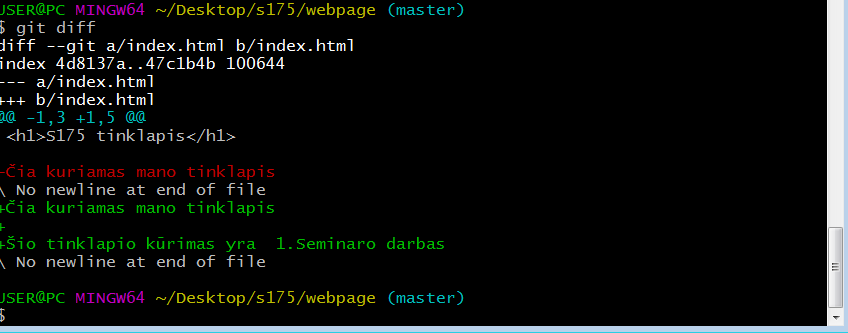
\includegraphics[scale=0.4]{webpage_4.png}
\end{figure}

\item Kadangi pakeitimai teisingi, galima \colorbox{listinggray}{\lstinline|git commit -am "Sukurta index.html antraštė"|}. Kadangi jau trackinam visus failus tai galima naudoti sutrumpintą komandą, kur -am reiškia -all ir -m

\item Na bet į internetinį puslapį toli gražu tai dar nepanašu... Todėl į editorių perrašome šį bloką" (arba pradedame typinti <h ir pasirenkame html ir užpildome trūkstama informacija)

\begin{lstlisting}
<!DOCTYPE html>
<html>
<head>
	<title>Home</title>
</head>
<body>
<h1>S175 Tinklaps</h1>
<p>Čia kuriamas mano tinklapis</p>
<p>Šio tinklapio kūrimas yra 1.Seminaro darbas </p>
</body>
</html>
\end{lstlisting}

\begin{itemize}
\item \colorbox{listinggray}{\lstinline|<!DOCTYPE html>|} nusako koks tai dokumento tipas, šiuo atveju tai html dokumentas
\item \colorbox{listinggray}{\lstinline|<html>|} atidaro html tag
\item \colorbox{listinggray}{\lstinline|<head>|} atidaro head tag
\item \colorbox{listinggray}{\lstinline|	<title></title>|} atidaro ir uždaro title tag
\item \colorbox{listinggray}{\lstinline|</head>|} uždaro head  tag
\item \colorbox{listinggray}{\lstinline|<body>|} atidaro body tag (t.y. puslapio turinys)
\item \colorbox{listinggray}{\lstinline|<h1></h1>|} atidaro ir uždaro anntraštės tipo tag
\item \colorbox{listinggray}{\lstinline|<p></p>|} atidaro ir uždaro paragrafo tag
\item \colorbox{listinggray}{\lstinline|</body>|} uždaro body tag
\item \colorbox{listinggray}{\lstinline|</html>|} uždaro html tag
\end{itemize}


\begin{figure}[H]
\center
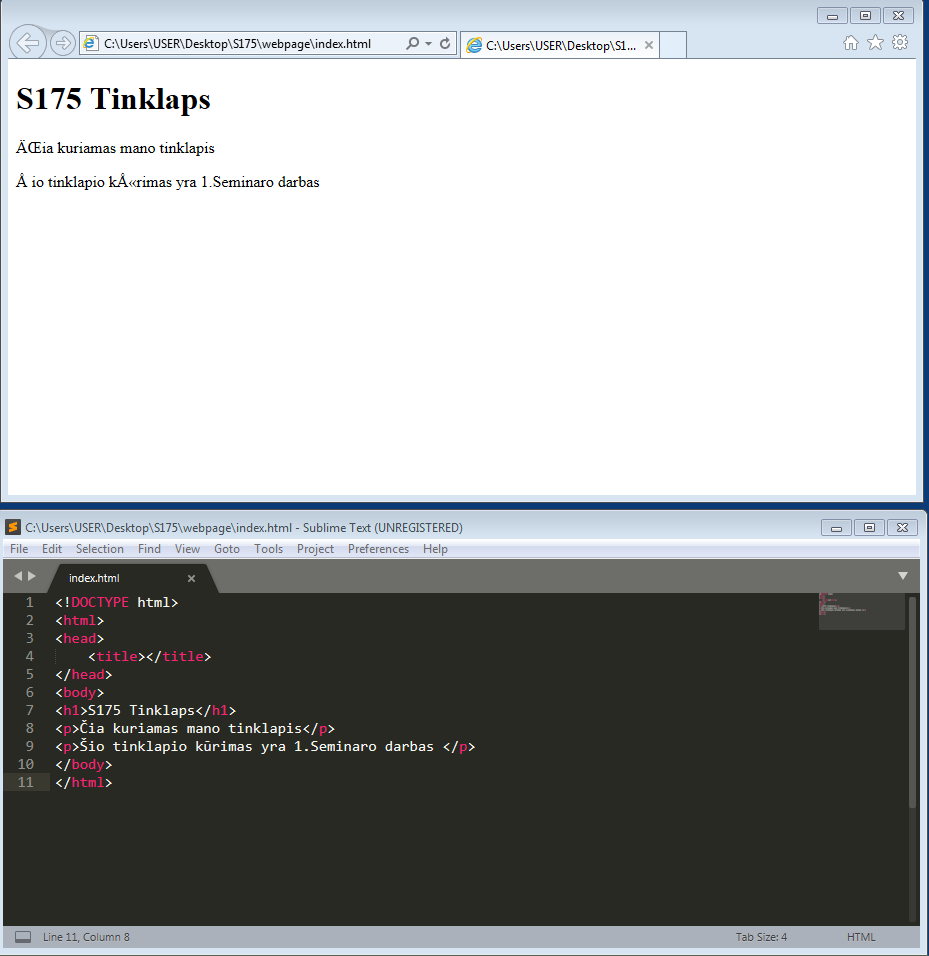
\includegraphics[scale=0.4]{webpage_5.png}
\end{figure}

\item Matyti, jog naršyklėje esantis Tab rodo ne visai tai, ką norėtume matyti, pvz., "Home", todėl turime editoriaus kodą 4 eilutėje pakeist į \colorbox{listinggray}{\lstinline|<title>Home</title>|}

\item Dar vienas nemalonus dalykas, naršyklė nesupranta lietuviškų simbolių, todėl įterpiame  po pirmos eilutės: \colorbox{listinggray}{\lstinline|<meta charset="utf-8"/>|}, taigi priskiriame meta informaciją puslapiui ir pasakome, jog naršyklė skaitydama šį tekstą naudotų utf-8 kodavimą, kuris turi ir lietuviškus simbolius

\item Išsaugome editoriaus pakeitimus, atnaujiname naršyklę ir  commitinam pakeitimus \colorbox{listinggray}{\lstinline|git commit -am "papildytas index.html"|}.  Dabartinis tinklapis jau daug maž panašus į tinklapį.

\begin{figure}[H]
\center
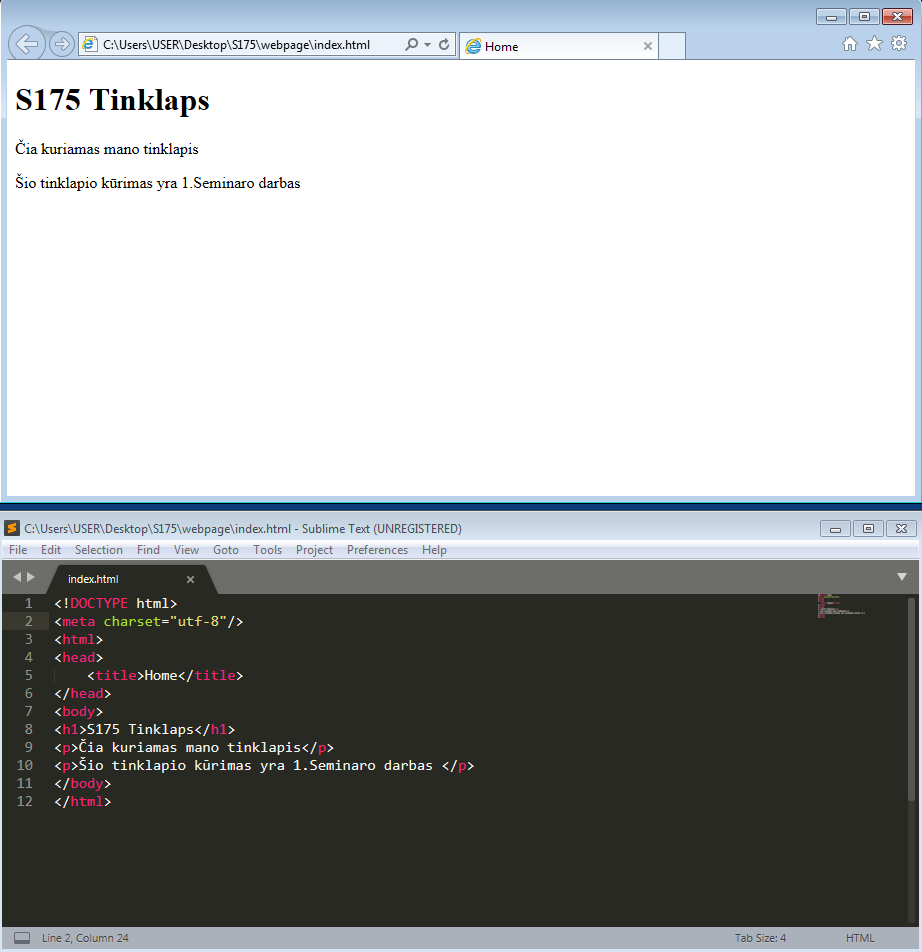
\includegraphics[scale=0.4]{webpage_6.png}
\end{figure}

\item Github sukuriame naują repo "webpage", Praleidžiame aprašymą ir paliekame be "README".

\item Keliaujame į Git Bash ir įrašome

\colorbox{listinggray}{\lstinline|git remote add origin https://github.com/vartotojovardas/webpage.git"|}.

tada shipinam savo darbą į internetą:

\colorbox{listinggray}{\lstinline|git push -u origin master"|}. -u reiškia, jog vietinė repo išmoksta, kad \textit{Github} yra \textit{upstream repository}, o tai leis ateityje tiesiog parsisiųsti naudojant \textit{pull} komandą. Ataujiname Github psl ir pamatysim

\begin{figure}[H]
\center
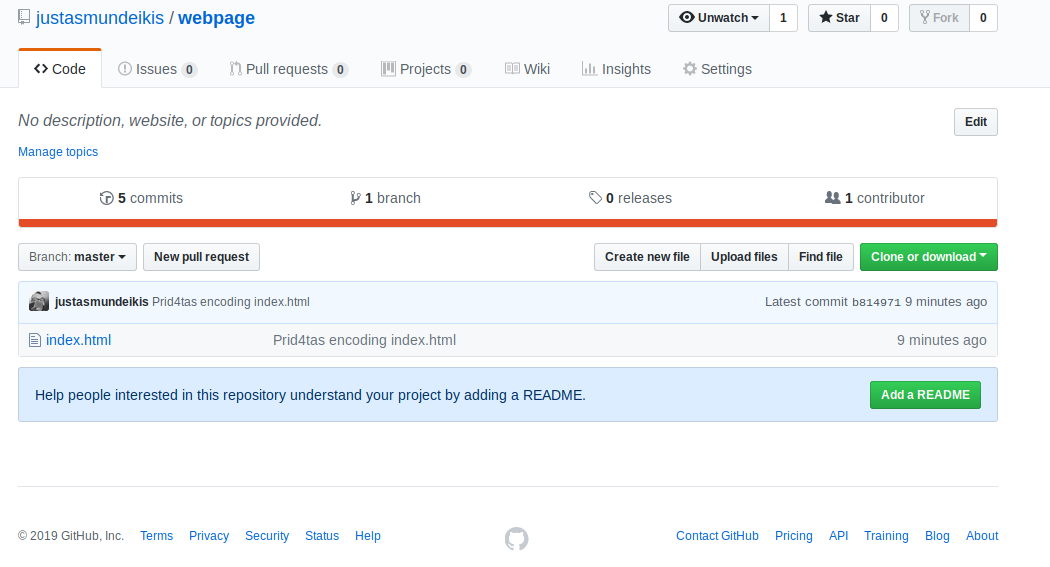
\includegraphics[scale=0.4]{webpage_7.png}
\end{figure}

\item Kadangi nėra blogai turėti README failą, tai Git Bash sukuriame ji.

\colorbox{listinggray}{\lstinline|touch README.md"|}.

o tada atsidarome failą su \textit{Sublime} ir perrašome šį Markdown formatuotą tekstą:

\begin{lstlisting}
# Bandomasis puslapis

Čia kuriamas bandomasis puslapis. Ši paskyra priklauso studentui S.... 
Šis puslapis kurimas Vilniaus Universiteto Ekonomikos ir verslo administravimo fakultete vykstančios **"Duomenų analizės įvado"** paskaitų metu
\end{lstlisting}

\item dabar reikia stag'inti ir commit'inti  README.md fail, bei ship'inti jį į Github


\colorbox{listinggray}{\lstinline|git add . && git commit -m "sukurtas README.md"|} bei

\colorbox{listinggray}{\lstinline|git push|}. Kadangi jau pasakėme kas yra \textit{upstream repository}, galime trumpinti komandą.

\item Atnaujinius GitHub puslapį, matome:

\begin{figure}[H]
\center
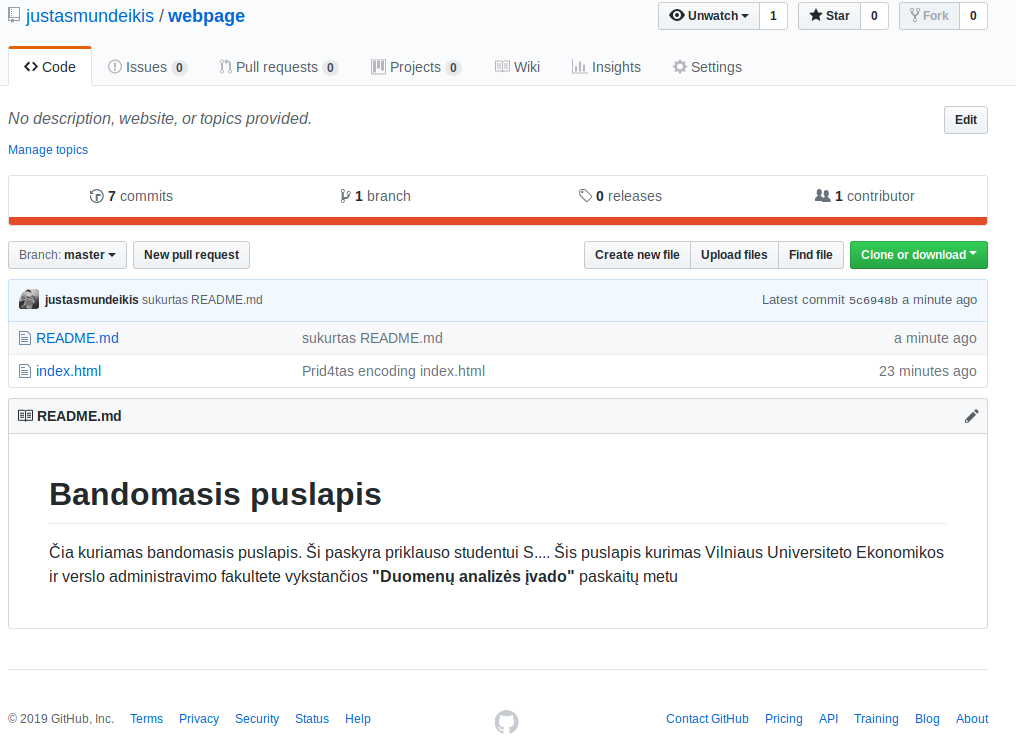
\includegraphics[scale=0.4]{webpage_8.png}
\end{figure}



\item Čia galima rasti daugiau markdown formativimo subtilybių: \href{https://guides.github.com/pdfs/markdown-cheatsheet-online.pdf}{\color{blue}{Markdown cheetsheat link}}

\item Kadangi puslapis yra gana nykus, pabandysim įdėti kokį linksmą paveiksliuką

\item Git Bash sukuriame naują aplanką \colorbox{listinggray}{\lstinline|mkdir images|}
\item Git Bash yra stiprus tuo, jog gali netgi atsiųsti failus iš interneto! Tam naudojame šią komandą: 

\colorbox{listinggray}{\lstinline|curl -o images/github.png -OL https://upload.wikimedia.org/wikipedia/commons/thumb/b/b3/GitHub.svg/567px-GitHub.svg.png
|}

Folderyje images turėjo atsirasti šis paveiksliukas

\begin{figure}[H]
\center

\includegraphics[scale=0.2]{github.png}
\end{figure}

\item Dabar reikia dar jį įterpti į \textit{index.html} failą. Tai galime padaryti html body įrašę tokią eilutę \colorbox{listinggray}{\lstinline|<img src="path/to/file" alt="Description">|}. Kadangi paveiksliukas yra \textit{images} tai įrašome atitinkamai src="" (source). Na bet kad būtų linksmiau, pridedame dar ir  vieną paveikklsiuk iš interneto 

\begin{lstlisting}
<!DOCTYPE html>
<meta charset="utf-8"/>
<html>
<head>
	<title>Home</title>
</head>
<body>
<h1>S175 Tinklaps</h1>
<p>Čia kuriamas mano tinklapis</p>
<p>Šio tinklapio kūrimas yra 1.Seminaro darbas </p>
<p><img src="images/github.png" alt="github paveiksliukas"></p>
<p><img src="https://studyguide.itu.dk/~/media/studyguide/student-life/facilities-at-itu/it-facilities/github/github_logo.png?h=248&w=573&la=en">
</p>
</body>
</html>
\end{lstlisting}

\colorbox{listinggray}{\lstinline|git add . && git commit -m "pridėti paveiksliukai.md"|} bei

\colorbox{listinggray}{\lstinline|git push|}

Ataujinus Github puslapį, matome, jog atsirado folderis "images"

\begin{figure}[H]
\center
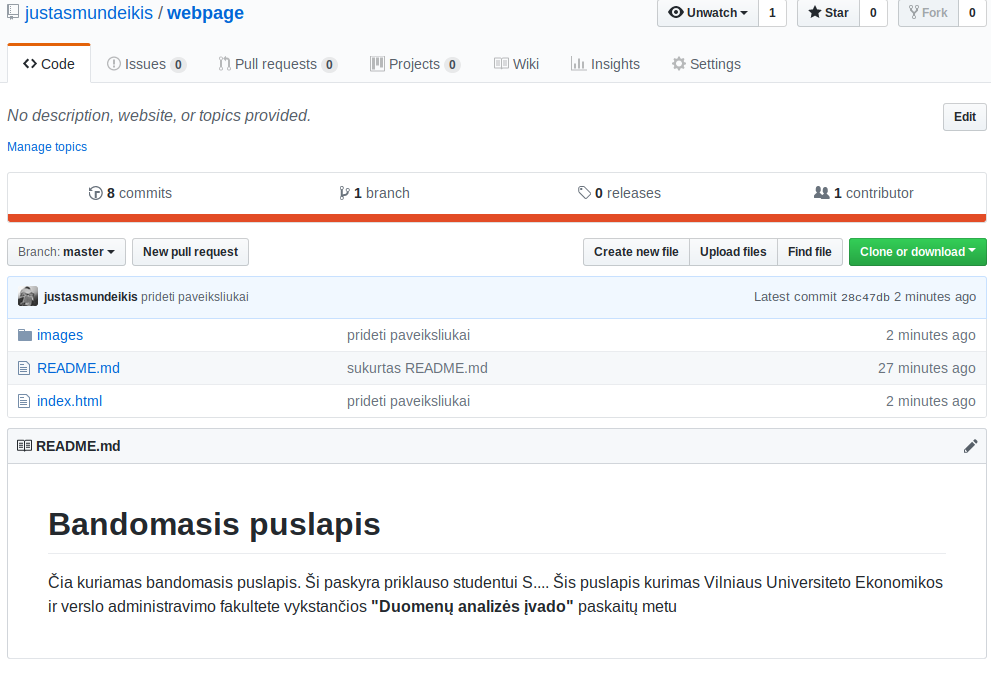
\includegraphics[scale=0.4]{webpage_9.png}
\end{figure}

\item GitBash sukuriame naują atšaką ir einame į ją \colorbox{listinggray}{\lstinline| git checkout -b about-puslapis|} [-b sukuria atšaką]. Alternatyviai \colorbox{listinggray}{\lstinline| git brancha about-puslapis|} ir \colorbox{listinggray}{\lstinline| git checkout about-puslapis|}
 
\item Nukopijuojame index.html į failą pavadinimu about.html naudodami komandą
\colorbox{listinggray}{\lstinline|cp index.html about.html|}

\item Atsidarome about.html su Sublime ir pakeičiame turinį, supildant savo duomenis

\begin{lstlisting}
<!DOCTYPE html>
<meta charset="utf-8"/>
<html>
<head>
	<title>About</title>
</head>
<body>
<p><strong>Vardas:</strong> Vardas Pavardė</p>
<p><strong>Stud. nr.:</strong> S175</p>
<p><strong>Kursas</strong>: Ekonomika</p>
<p><strong>Grupė:</strong> xx</p>
</body>
</html>
\end{lstlisting}

\item Kadangi norime, jog ir pagrindiniame puslapyje būtų nuorodą į puslapi apie mus, turime pakeisti index.html į

\begin{lstlisting}
<!DOCTYPE html>
<meta charset="utf-8"/>
<html>
<head>
	<title>Home</title>
</head>
<body>
<h1>S175 Tinklaps</h1>
<p>Čia kuriamas mano tinklapis</p>
<p>Šio tinklapio kūrimas yra 1.Seminaro darbas </p>
<br>
<a href="about.html">Daugiau informacijos apie mane</a>
<p><img src="images/github.png" alt="github paveiksliukas"></p>
<p><img src="https://studyguide.itu.dk/~/media/studyguide/student-life/facilities-at-itu/it-facilities/github/github_logo.png?h=248&w=573&la=en">
</p>
</body>
</html>
\end{lstlisting}

taigi įterpiame \colorbox{listinggray}{\lstinline|<a href="about.html">Daugiau informacijos apie mane</a>|}, tagas <a> reiškia "anchor" arba "inkaras" ir yra  naudojamas nuorodoms. 

\item \colorbox{listinggray}{\lstinline|git add . && git commit -m "sukurtas about.html puslapis"|}  

\item Tačiau esame atšakoje "about-puslpis", todėl grįžtame į "master" su \colorbox{listinggray}{\lstinline|git checkout master|}. Jame suprantama nėra pakeitimų, kurios padarėme atšakoje, todėl nusprendžiame sjingti atšaką su master naudodami komandą
\colorbox{listinggray}{\lstinline|git merge about-puslapis|}.

\item Jeigu nėra kokių nors jungimo klaidų, kurias reiktų pataisyti ranka, nuostabu!

\item Jeigu nebereikia about-puslapis atšakos, kuri yra sujungta (merge), galime ją ištrinti: \colorbox{listinggray}{\lstinline|git branch -d about-puslapis|}. 

\item Jeigu būtume sukūrę atšaką, bet joje nieko prasmingo nesukūrė,flag -d neleistų ištrinti atšakos, tada reiktų naudoti flag -D, pvz.,  \colorbox{listinggray}{\lstinline|git branch -D about-puslapis|}. 

\item pasitikriname kiek atšakų turime su  \colorbox{listinggray}{\lstinline|git branch|}.

\item Dabar galima \item \colorbox{listinggray}{\lstinline|git push|}. Po sujungimo staginti ir commitinti nebereikia, nes staginimas ir commitinimas įvyko dar about-puslapis atšakoje!

\item dabar reikia nueiti į "Settings" 
\begin{figure}[H]
\center
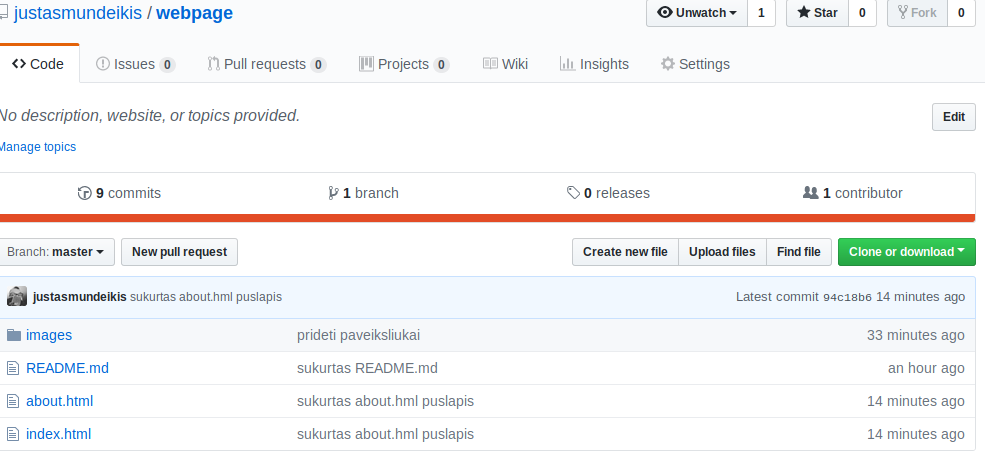
\includegraphics[scale=0.4]{webpage_10.png}
\end{figure}

\item Ties "GitHub Pages" iš "None" pasikeisti į "master branch"

\begin{figure}[H]
\center
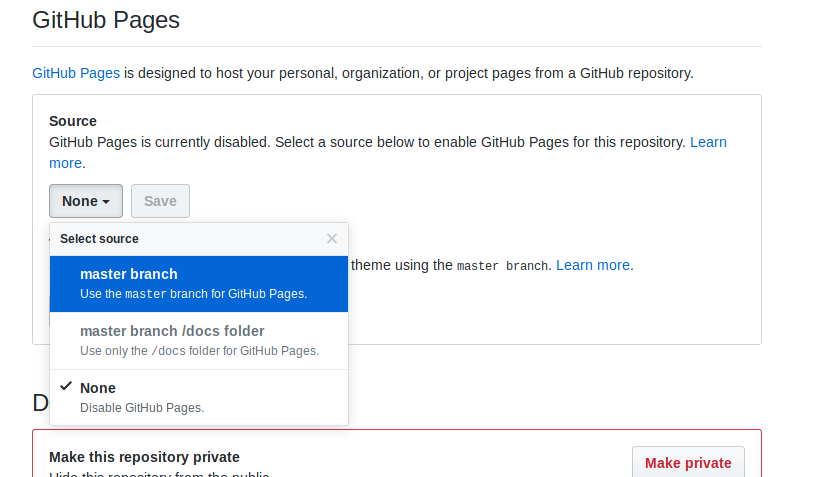
\includegraphics[scale=0.4]{webpage_11.png}
\end{figure}

\item Paspaudus nuorodą:
\begin{figure}[H]
\center
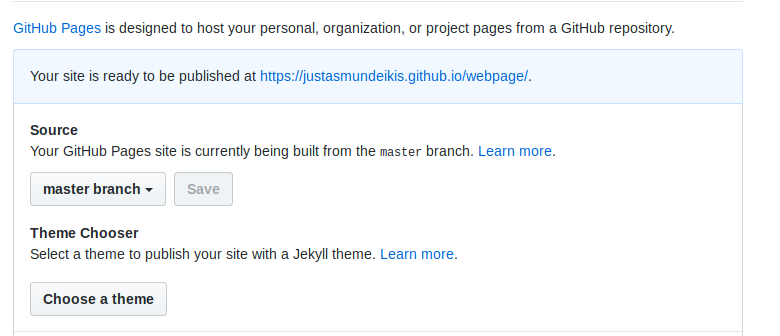
\includegraphics[scale=0.4]{webpage_12.png}
\end{figure}
 
\item Atsidaro pilnai veikiantis tinklapis! Sveikinu!
\begin{figure}[H]
\center
\fbox{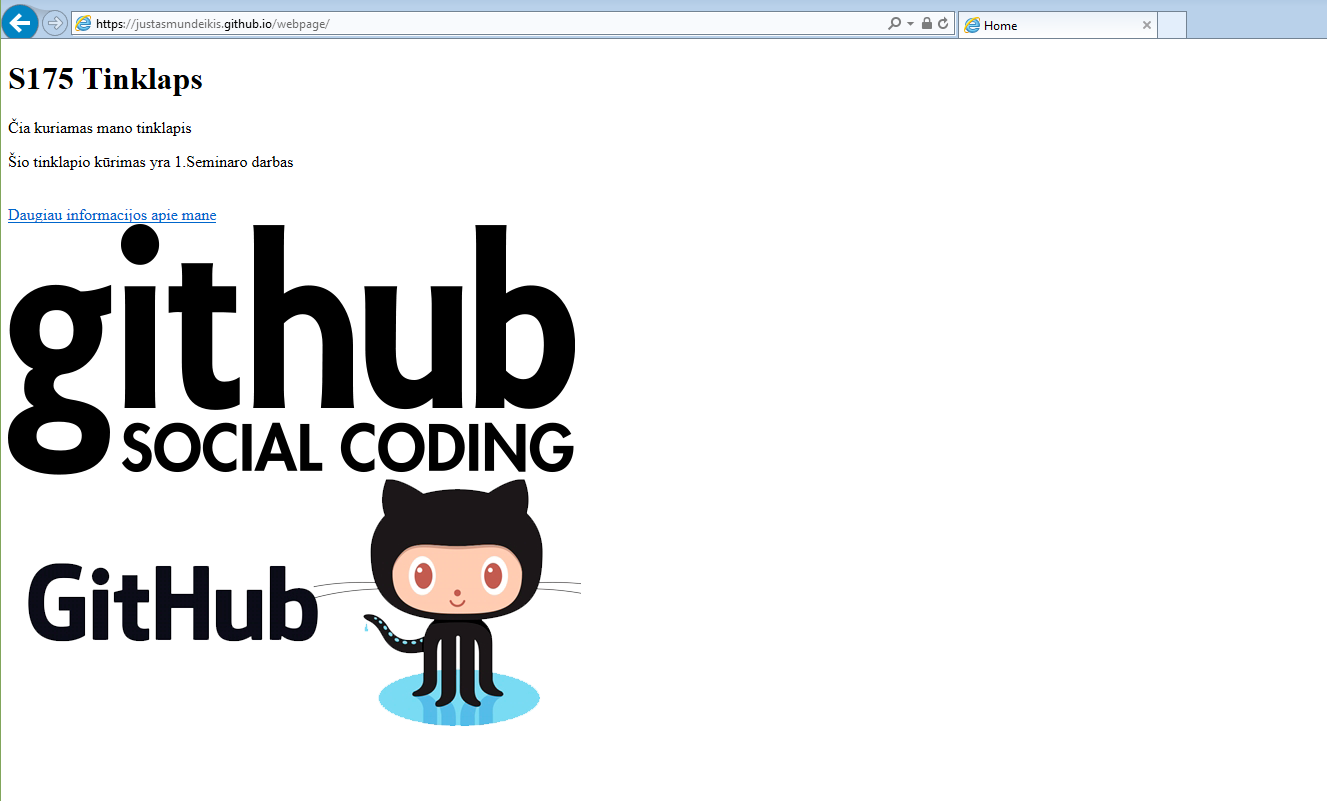
\includegraphics[scale=0.3]{webpage_13.png}}
\end{figure}
 
 
\item Jeigu norite sukurti labiau sofistikuotą puslapį, galima naudotis html editoriaus pagalba, pvz., https://html-online.com/editor/


\section{Kaip sukruti nuosavą homepage per 5 min}
\begin{itemize}
\item Github paskyroje sukuriame naują \textit{repo} pvz., "webpage2"
\item Parsisiunčiam iš tinklapio https://designseer.com/free-blog-html-css-templates/ "KeepSimple" tinklapio paketą išsaugant jį S175 folderyje
\item Unzipiniam atsisiųstą failų paketą su GitBash \colorbox{listinggray}{\lstinline|unzip KeepItSimple20.zip|}
\item Pereinam į išpakuotą folderį, inicializuojame git, pridedame visus failus, ir commitiname naudojant sujungtą komandą:

\colorbox{listinggray}{\lstinline|cd KeepSimple20 && git init && git add . && git commit -m "sukelti failai"|}
\item sujungiame su Github
\colorbox{listinggray}{\lstinline|git remote add origin https://github.com/<username>/webpage2.git"|}
\item ir pushinam į Github \colorbox{listinggray}{\lstinline|git push -u origin master"|}
\item "Settings" esančioje "GitHub pages" dalyje, "Source" pakeičiame į "master"
\item ir nuspaudus ant nuorodos turime veikiantį tinklapį

\begin{figure}[H]
\center
\fbox{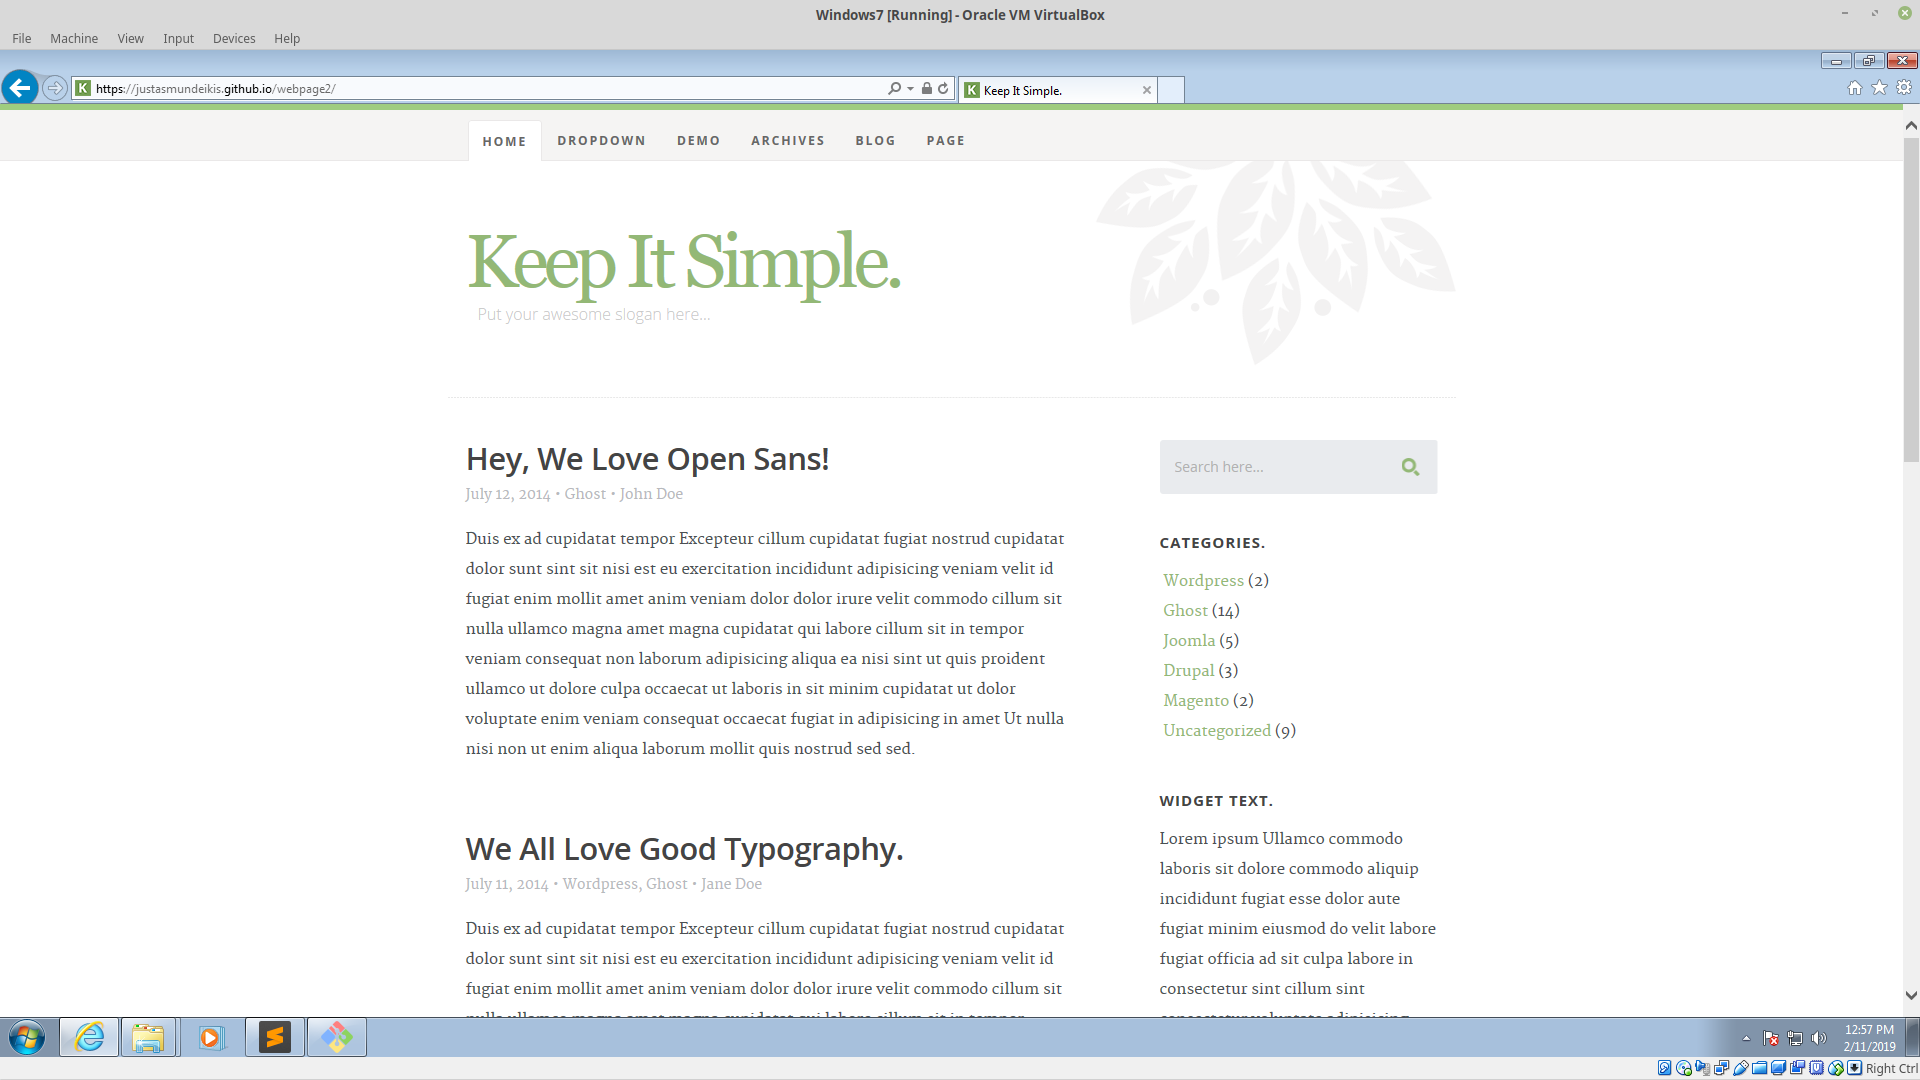
\includegraphics[scale=0.2]{webpage_14.png}}
\end{figure}

\item tiesa, jis kiek sudėtingesnis, turi Java Script, CSS ir t.t., bet pati struktūra yra aiški
\item Kuo paprastesnį Template susirasite, tuo papračiau galima turėti savo tinklapį ir jį keisti
\item Taip pat puslapį galima susikurti ir tiesiog pačiame Github

\end{itemize}













\end{enumerate}
\end{document}